\documentclass[11pt]{article}
\usepackage{cmap}

% ---------------------------------------------------------------------------
% Reusable course-notes template
%
% Edit this metadata block for every course or document.
% Keep the braces, and replace only the text inside them.
% ---------------------------------------------------------------------------
\newcommand{\CourseName}{GoTrain}
\newcommand{\CourseNumber}{AUB ACM $\times$ RASID Hackathon}
\newcommand{\AuthorName}{Team 8: Charbel, Marwa and Rabih}
\newcommand{\DocumentTopic}{Technical Report for the Jury}

\usepackage[letterpaper,margin=1in]{geometry}
\usepackage[T1]{fontenc}
\usepackage{lmodern}
\usepackage{microtype}
\usepackage{amsmath,amssymb,mathtools}
\usepackage{xcolor}
\usepackage{fancyhdr}
\usepackage{graphicx}
\usepackage{booktabs}
\usepackage{tabularx}
\usepackage{array}
\usepackage{enumitem}
\usepackage{tikz}
\usetikzlibrary{arrows.meta,positioning}
\usepackage{pgfplots}
\pgfplotsset{compat=1.17}
\usepgfplotslibrary{groupplots}
\usepackage[hidelinks]{hyperref}

% Keep PDF bookmarks plain even when the visible contents use custom formatting.
\pdfstringdefDisableCommands{%
  \def\tocsectionentry#1#2{#1 #2}%
  \def\tocsubsectionentry#1#2{#1 #2}%
}

\definecolor{boxgray}{gray}{0.94}
\definecolor{rulegray}{gray}{0.55}
\definecolor{wine}{RGB}{128,0,32}
\definecolor{winelight}{RGB}{176,40,79}
\definecolor{rose}{RGB}{240,169,187}

\setlength{\parindent}{0pt}
\setlength{\parskip}{0.55em}
\allowdisplaybreaks
\setlist{itemsep=0.15em,topsep=0.3em}
\newcolumntype{Y}{>{\raggedright\arraybackslash}X}
\newcommand{\run}[1]{\texttt{\small #1}}
\newcommand{\up}[1]{\textcolor{wine}{\textbf{#1}}}

% ---------------------------------------------------------------------------
% Header / footer
% ---------------------------------------------------------------------------
\pagestyle{fancy}
\fancyhf{}
\fancyhead[L]{\small\CourseNumber}
\fancyhead[C]{\small\DocumentTopic}
\fancyhead[R]{\small\CourseName}
\fancyfoot[C]{\thepage}
\renewcommand{\headrulewidth}{0.4pt}
\renewcommand{\footrulewidth}{0pt}

% ---------------------------------------------------------------------------
% Section and contents styling
% ---------------------------------------------------------------------------
\makeatletter
\newcommand{\tocsectionentry}[2]{\textbf{#1)\quad #2}}
\newcommand{\tocsubsectionentry}[2]{#1)\quad #2}
\newcommand{\tocleaders}{%
  \nobreak\leaders\hbox{$\m@th\mkern\@dotsep mu.\mkern\@dotsep mu$}\hfill\nobreak
}
\renewcommand*\l@section[2]{%
  \ifnum\c@tocdepth>\z@
    \addpenalty{\@secpenalty}%
    \addvspace{0.35em}%
    \begingroup
      \parindent\z@
      \rightskip\@pnumwidth
      \parfillskip-\@pnumwidth
      \leavevmode #1\tocleaders\hb@xt@\@pnumwidth{\hfil\bfseries #2}\par
    \endgroup
  \fi
}
\renewcommand*\l@subsection[2]{%
  \ifnum\c@tocdepth>\@ne
    \begingroup
      \parindent\z@
      \rightskip\@pnumwidth
      \parfillskip-\@pnumwidth
      \leavevmode\hspace*{2.25em}#1\tocleaders\hb@xt@\@pnumwidth{\hfil #2}\par
    \endgroup
  \fi
}
\newcommand{\CourseTableOfContents}{%
  \begingroup
    \@starttoc{toc}%
  \endgroup
}
\makeatother

\newcommand{\coursesection}[1]{%
  \refstepcounter{section}%
  \setcounter{subsection}{0}%
  \addcontentsline{toc}{section}{\protect\tocsectionentry{\thesection}{#1}}%
  \par\vspace{2.0em}%
  \noindent
  {\fontsize{24}{26}\selectfont\bfseries\color{black}\thesection}%
  \hspace{0.65em}%
  {\color{rulegray}\vrule width 0.6pt height 1.75em depth 0.25em}%
  \hspace{0.65em}%
  {\Large\bfseries #1\par}%
  \vspace{0.2em}{\color{rulegray}\hrule height 0.4pt}\vspace{0.9em}%
}

\newcommand{\coursesubsection}[1]{%
  \refstepcounter{subsection}%
  \addcontentsline{toc}{subsection}{\protect\tocsubsectionentry{\thesubsection}{#1}}%
  \par\vspace{1.25em}%
  \noindent{\large\bfseries\thesubsection)\hspace{0.7em}#1\par}%
  \vspace{0.55em}%
}

\renewcommand{\section}[1]{\coursesection{#1}}
\renewcommand{\subsection}[1]{\coursesubsection{#1}}

\newcommand{\ContentsTitle}{%
  \vspace{0.55em}
  \begin{center}
    \fbox{\parbox{0.86\linewidth}{\centering\Large\bfseries Contents}}
  \end{center}
  \vspace{-1.15em}
}

% ---------------------------------------------------------------------------
% Mathematical environments (definitions are the only boxed blocks)
% ---------------------------------------------------------------------------
\newcounter{definition}[section]
\newcounter{theorem}[section]
\newcounter{corollary}[section]
\newcounter{example}[section]
\newcounter{remark}[section]
\renewcommand{\thedefinition}{\thesection.\arabic{definition}}
\renewcommand{\thetheorem}{\thesection.\arabic{theorem}}
\renewcommand{\thecorollary}{\thesection.\arabic{corollary}}
\renewcommand{\theexample}{\thesection.\arabic{example}}
\renewcommand{\theremark}{\thesection.\arabic{remark}}

\newsavebox{\noteboxcontent}
\newenvironment{notebox}[2]{%
  \par\addvspace{0.85em}%
  \begingroup
  \def\noteboxfill{#2}%
  \setlength{\fboxsep}{8pt}%
  \begin{lrbox}{\noteboxcontent}%
    \begin{minipage}{\dimexpr\linewidth-2\fboxsep-2\fboxrule\relax}%
    \textbf{#1}\quad%
}{%
    \end{minipage}%
  \end{lrbox}%
  \noindent\fcolorbox{black}{\noteboxfill}{\usebox{\noteboxcontent}}%
  \endgroup
  \par\addvspace{0.85em}%
}

\newenvironment{definition}[2]{%
  \refstepcounter{definition}\label{def:#2}%
  \begin{notebox}{Definition \thedefinition\ (#1).}{boxgray}%
}{\end{notebox}}

\newenvironment{theorem}[2]{%
  \refstepcounter{theorem}\label{thm:#2}%
  \par\addvspace{0.85em}%
  \noindent\textbf{Theorem \thetheorem\ (#1).}\quad\itshape
}{%
  \par\addvspace{0.85em}%
}

\newenvironment{corollary}[2]{%
  \refstepcounter{corollary}\label{cor:#2}%
  \par\addvspace{0.85em}%
  \noindent\textbf{Corollary \thecorollary\ (#1).}\quad\itshape
}{%
  \par\addvspace{0.85em}%
}

\newenvironment{examplebox}{%
  \refstepcounter{example}%
  \par\addvspace{0.85em}%
  \noindent\textbf{Example \theexample.}\quad
}{%
  \par\addvspace{0.85em}%
}

\newenvironment{remarkbox}{%
  \refstepcounter{remark}%
  \par\addvspace{0.85em}%
  \noindent\textit{Remark \theremark.}\quad
}{%
  \par\addvspace{0.85em}%
}

\newcommand{\divider}{\par\vspace{0.6em}{\color{rulegray}\hrule height 0.4pt}\vspace{0.6em}}

% Only main sections in the contents so that it fits on the title page.
\setcounter{tocdepth}{1}

\begin{document}
\pagenumbering{roman}

\begin{titlepage}
  \thispagestyle{empty}
  \centering
  \vspace*{0.05in}

  {\huge\bfseries \CourseName\par}
  \vspace{0.25em}
  {\large An autonomous AI scientist that trains geospatial models on its own\par}
  \vspace{0.35em}
  {\LARGE\CourseNumber\par}
  \vspace{0.25em}
  {\Large By \AuthorName\par}

  \vspace{0.45em}
  {\color{rulegray}\rule{0.78\linewidth}{0.5pt}\par}
  \vspace{0.4em}
  {\Large\itshape \DocumentTopic\par}

  \vspace{0.8em}
  \begin{tabular}{@{}cccc@{}}
    \textbf{\Large 95.7\%} & \textbf{\Large 97.9\%} & \textbf{\Large 0.951} & \textbf{\Large 0.844} \\
    \small EuroSAT accuracy & \small PV4GER accuracy & \small PV4GER-seg mIoU & \small NZ-cattle mIoU
  \end{tabular}\par
  \vspace{0.2em}
  {\small Final test scores, each test split opened exactly once. About 64 GPU-minutes on one Tesla T4.\par}

  \ContentsTitle
  {\normalsize\linespread{1.05}\selectfont\CourseTableOfContents}
\end{titlepage}
\clearpage
\pagenumbering{arabic}

% ===========================================================================
\section{Executive Summary}
% ===========================================================================

Earth-observation models are still built by hand: an expert picks a backbone,
designs a training recipe and tunes it, again for every new sensor and task.
\textbf{GoTrain} replaces that loop with an agent. Given a GEO-Bench dataset and a
GPU budget, a Strands agent driven by Claude Sonnet on Amazon Bedrock inspects
the data, states a hypothesis, trains a model on the SageMaker GPU, measures it on
the validation split, and decides what to try next. Every decision is logged, and
the test split is opened exactly once, at the end, by a separate locked command.

\begin{table}[h]
\centering
\caption{Final test results. Selection used validation data only; each test split was evaluated once.}
\label{tab:headline}
\begin{tabular}{@{}llrrrr@{}}
\toprule
Task & Type & Test images & Metric & Final test & Best validation \\
\midrule
\texttt{m-eurosat} & 10-class classification & 1{,}000 & accuracy & \textbf{95.70\%} & 97.20\% \\
\texttt{m-pv4ger} & binary classification & 999 & accuracy & \textbf{97.90\%} & 97.50\% \\
\texttt{m-pv4ger-seg} & binary segmentation & 403 & mean IoU & \textbf{0.9514} & 0.9526 \\
\texttt{m-nz-cattle} & binary segmentation & 65 & mean IoU & \textbf{0.8439} & 0.8476 \\
\bottomrule
\end{tabular}
\end{table}

What we want the jury to remember:
\begin{enumerate}
  \item \textbf{Strong scores from a disciplined process.} A manual CNN reached 75\% on
  EuroSAT; the agent's pipeline reached 97\% validation and 95.7\% test. Validation and
  test agree closely on three of four tasks, which indicates we did not overfit to validation.
  \item \textbf{Every gain is explained by a measured hypothesis.} For example, the agent
  noticed that cattle cover only 2.2\% of pixels and raised the input resolution
  (+0.014 mIoU); it noticed 36 missed solar panels and turned on class balancing
  (+1.0 point accuracy).
  \item \textbf{An AI scientist, not a tuner.} GoTrain diagnoses where a model fails
  (object detection rate by size, confused classes, worst images), proposes a targeted fix,
  keeps it only if validation improves, and \textbf{remembers} the outcome across datasets.
  \item \textbf{Production-minded.} Immutable model versions with SHA-256 checksums, a model
  registry with verified restores, a ChatGPT-style interface, a results dashboard, 34
  automated tests and an MCP server so that GoPilot can call the same tools.
\end{enumerate}

% ===========================================================================
\section{The Challenge and Our Ground Rules}
% ===========================================================================

\subsection{The four problems we chose}

The brief asked for two classification and two segmentation problems from GEO-Bench.
We chose them to cover different sensors and difficulty levels.

\begin{table}[h]
\centering
\caption{Selected GEO-Bench tasks (split sizes from the brief; class balance measured on a seeded training sample).}
\begin{tabularx}{\linewidth}{@{}lYrrl@{}}
\toprule
Task & What is predicted & Train / val / test & Input & Imbalance \\
\midrule
\texttt{m-eurosat} & land cover, 10 classes & 2000 / 1000 / 1000 & Sentinel-2, 13 bands & roughly balanced \\
\texttt{m-pv4ger} & solar panel present or not & 11814 / 999 / 999 & aerial RGB, 0.1 m & 15.6\% positive \\
\texttt{m-pv4ger-seg} & solar panel pixels & 3000 / 403 / 403 & aerial RGB, 0.1 m & 19.2\% foreground \\
\texttt{m-nz-cattle} & cattle pixels & 524 / 66 / 65 & aerial RGB, 0.1 m & \textbf{2.2\% foreground} \\
\bottomrule
\end{tabularx}
\end{table}

\subsection{The one rule we enforced in code, not in discipline}

\begin{definition}{Protocol}{protocol}
The \emph{train} split fits weights. The \emph{valid} split is the only signal used to
choose recipes, epochs and checkpoints. The \emph{test} split is opened once per task,
after the selected model has been frozen, and never influences any decision.
\end{definition}

We did not rely on good intentions. The development data loader refuses any split
other than \texttt{train} and \texttt{valid}; the agent and the MCP server have no
test tool at all; and \texttt{gotrain finalize} freezes the best validation run,
creates an exclusive marker file \emph{before} opening the first test sample, and
refuses to run twice (Section~\ref{sec:integrity}).

% ===========================================================================
\section{System Architecture}
% ===========================================================================

\begin{figure}[h]
\centering
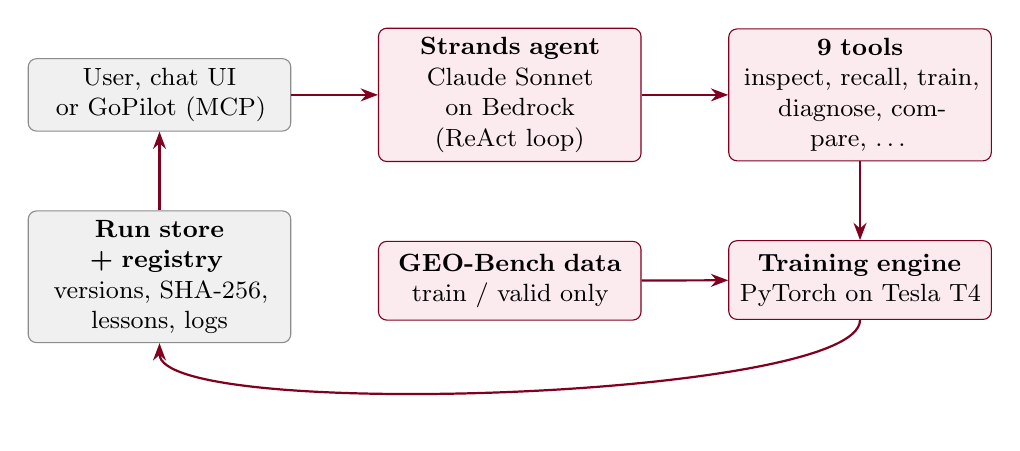
\begin{tikzpicture}[
  box/.style={draw=wine, rounded corners=3pt, fill=rose!25, align=center, minimum height=1.0cm, text width=3.1cm, font=\small},
  side/.style={draw=rulegray, rounded corners=3pt, fill=boxgray, align=center, minimum height=0.9cm, text width=3.1cm, font=\small},
  arr/.style={-{Stealth[length=2.2mm]}, thick, color=wine}]
  \node[side] (user) {User, chat UI\\or GoPilot (MCP)};
  \node[box, right=1.1cm of user] (agent) {\textbf{Strands agent}\\Claude Sonnet on Bedrock\\(ReAct loop)};
  \node[box, right=1.1cm of agent] (tools) {\textbf{9 tools}\\inspect, recall, train,\\diagnose, compare, \dots};
  \node[box, below=1.0cm of tools] (engine) {\textbf{Training engine}\\PyTorch on Tesla T4};
  \node[box, below=1.0cm of agent] (data) {\textbf{GEO-Bench data}\\train / valid only};
  \node[side, below=1.0cm of user] (store) {\textbf{Run store + registry}\\versions, SHA-256,\\lessons, logs};
  \draw[arr] (user) -- (agent);
  \draw[arr] (agent) -- (tools);
  \draw[arr] (tools) -- (engine);
  \draw[arr] (data) -- (engine);
  \draw[arr] (engine.south) .. controls +(0,-1.0) and +(0,-1.0) .. (store.south);
  \draw[arr] (store) -- (user);
\end{tikzpicture}
\caption{GoTrain at a glance. The agent reasons; the tools act; every result lands in an immutable, checksummed run store.}
\label{fig:arch}
\end{figure}

\subsection{Components}

\begin{itemize}
  \item \textbf{Agent.} One Strands agent with a system prompt that encodes the protocol,
  sensible starting recipes and the scientist workflow (Section~\ref{sec:agent}). It runs a
  ReAct loop: reason, call a tool, read the measured result, reason again.
  \item \textbf{Tools.} \texttt{inspect\_dataset}, \texttt{recall\_lessons},
  \texttt{run\_experiment}, \texttt{diagnose\_errors}, \texttt{record\_lesson},
  \texttt{compare\_experiments}, \texttt{publish\_best\_model}, \texttt{publish\_dataset},
  \texttt{verify\_model\_download}. None of them can read the test split.
  \item \textbf{Training engine.} A single PyTorch pipeline for both problem types:
  data loading and caching, model construction, training with early stopping and a
  wall-clock budget, and validation metrics from a dataset-wide confusion matrix.
  \item \textbf{Storage.} Every run is an immutable directory named by timestamp and UUID
  containing its configuration, hypothesis, normalisation statistics, per-epoch history,
  event log, best checkpoint and SHA-256 hash. A registry publishes and restores versions
  with checksummed manifests.
  \item \textbf{Interfaces.} A command line, a chat web app (\texttt{gotrain ui}), an offline
  results dashboard, and a stdio MCP server exposing seven tools to GoPilot.
\end{itemize}

\subsection{Stack}

Python 3.12, PyTorch 2.7.1 and torchvision 0.22.1 (CUDA 12.6), geobench 1.1.0,
strands-agents 1.63.0, Claude Sonnet (\texttt{eu.anthropic.claude-sonnet-5-5},
\texttt{eu-central-1}), one NVIDIA Tesla T4 on Amazon SageMaker. Peak GPU memory of any
run was 1.2 GB, so the T4 was never the bottleneck.

% ===========================================================================
\section{Data Pipeline: Getting the Details Right}
% ===========================================================================

High accuracy starts with not corrupting the data. Each item below fixed or prevented a
real failure mode.

\subsection{Normalisation from training data only}

\begin{definition}{Train-only normalisation}{norm}
For each input channel $c$, the mean $\mu_c$ and standard deviation $\sigma_c$ are
estimated from a seeded random sample of 128 \emph{training} images at the training
resolution, and every input is transformed as $\tilde{x}_c = (x_c - \mu_c)/\sigma_c$.
The sampled indices are stored with each run, so the statistics are reproducible.
\end{definition}

We deliberately did not use benchmark-wide statistics: they can be computed on other
splits or a different band selection, which silently leaks information.

\subsection{Thirteen spectral bands into an ImageNet backbone}

EuroSAT has 13 Sentinel-2 bands, while pretrained ResNets expect 3. Rather than dropping
10 bands or training the first layer from scratch, we adapt the first convolution:

\begin{definition}{First-layer adaptation}{conv1}
Let $W\in\mathbb{R}^{64\times 3\times 7\times 7}$ be the pretrained first-layer weights.
For $C$ input channels the new weights are
\[
  W'_{:,c,:,:} \;=\; \frac{3}{C}\cdot\frac{1}{3}\sum_{j=1}^{3} W_{:,j,:,:}, \qquad c = 1,\dots,C,
\]
so that every band starts with the averaged RGB filters and the expected activation
magnitude matches what the pretrained network was trained on.
\end{definition}

We also found that EuroSAT's published band-name metadata is unreliable, so channels are
always used in their physical stored order and never selected by name.

\subsection{Augmentation that keeps masks aligned}

Training samples receive random horizontal and vertical flips and a random multiple of
$90^{\circ}$ rotation (the dihedral group of the square, a natural symmetry of nadir
imagery). For segmentation the identical transform is applied to the mask, which is
resized with nearest-neighbour interpolation so labels are never blended. A unit test
checks image and mask alignment.

\subsection{Evaluation at native label resolution}

Training may run on resized masks to fit the GPU, but validation and test predictions are
upsampled back to the \emph{native} annotation resolution before scoring, so the metric
is computed on the original labels.

\subsection{Throughput}

Resized development images are cached once as memory-mapped float16 tensors (when the
payload is below 2 GiB), while normalisation and random augmentation are still applied per
sample. With two data-loader workers overlapping I/O and GPU work, a full EuroSAT
training run takes about six minutes.

% ===========================================================================
\section{Models, Losses and Optimisation}
% ===========================================================================

\subsection{Architectures}

\begin{itemize}
  \item \textbf{Classification:} ImageNet-pretrained ResNet-18 or ResNet-34 with a new
  linear head (first layer adapted as in Definition~\ref{def:conv1}).
  \item \textbf{Segmentation:} a U-Net-style network with the pretrained ResNet as encoder.
  Four decoder stages upsample and concatenate the encoder skip connections
  ($512\to256\to128\to64\to32$ channels, GroupNorm, ReLU), followed by a
  $1\times1$ convolution and bilinear upsampling to the input size.
  \item A small randomly initialised CNN is kept for smoke tests and CPU checks.
\end{itemize}

\subsection{Loss functions}

\begin{definition}{Class-balanced cross-entropy}{balanced}
With $n_k$ training labels of class $k$ (pixels or images) and $N=\sum_k n_k$,
\[
  w_k = \operatorname{clip}\!\left(\frac{\sqrt{N/n_k}}{\tfrac1K\sum_j\sqrt{N/n_j}},\;0.1,\;10\right),
  \qquad
  \mathcal{L}_{\mathrm{CE}} = -\sum_i w_{y_i}\log p_{i,y_i} \Big/ \sum_i w_{y_i}.
\]
The square root softens the re-weighting, and clipping prevents extreme weights.
\end{definition}

\begin{definition}{Cross-entropy plus soft Dice (segmentation)}{dice}
With predicted probabilities $p_{k}$ and one-hot targets $y_{k}$ summed over the batch and pixels,
\[
  \mathcal{L} = \mathcal{L}_{\mathrm{CE}} + \frac{1}{K}\sum_{k=1}^{K}
  \left(1 - \frac{2\sum p_{k}y_{k} + 1}{\sum p_{k} + \sum y_{k} + 1}\right).
\]
Dice optimises region overlap directly and is far less dominated by the background
class than cross-entropy alone, which matters when the target covers 2\% of pixels.
\end{definition}

\subsection{Optimisation recipe}

AdamW (weight decay $10^{-4}$), cosine learning-rate annealing over the planned epochs,
gradient clipping at norm 5, optional mixed precision, and early stopping on the
validation metric with a configurable patience. Batch-norm running statistics of the
pretrained encoder are frozen during fine-tuning because small final batches made them
unstable. Every recipe is validated (allowed models, ranges for epochs, batch size, image
size and learning rate) before any GPU time is spent.

\subsection{Selection and inference}

\begin{definition}{Checkpoint selection}{selection}
After every epoch the model is scored on the validation split; the checkpoint with the
highest validation metric (accuracy for classification, mean IoU for segmentation) is
saved. Across runs, the selected model is $\arg\max$ of validation score; ties keep the
earlier run.
\end{definition}

\begin{definition}{Flip test-time augmentation (TTA)}{tta}
For the flip group $G=\{\mathrm{id},h,v,hv\}$, predictions are averaged in probability space,
\[
  \hat{p}(x) = \frac{1}{4}\sum_{g\in G} g^{-1}\!\big(\operatorname{softmax} f(g(x))\big),
\]
where $g^{-1}$ un-flips segmentation maps. It is adopted only if it wins on validation,
and it is recorded as a new, separate model version.
\end{definition}

\subsection{Metrics}

\begin{definition}{Dataset-wide IoU}{iou}
Let $C$ be the confusion matrix accumulated over \emph{all} validation (or test) pixels.
Then $\mathrm{IoU}_k = C_{kk}\,/\,(\sum_j C_{kj} + \sum_j C_{jk} - C_{kk})$, and mean IoU
averages over classes with non-empty union (background and foreground for binary tasks).
\end{definition}

Averaging per-batch IoUs would overweight small or empty images; the global confusion
matrix avoids that. We also report foreground IoU, balanced accuracy, macro-F1 and
per-class recall, and we never average accuracy with IoU across tasks.

% ===========================================================================
\section{The Agent: How GoTrain Decides}
\label{sec:agent}
% ===========================================================================

\subsection{One tool call is one experiment}

\texttt{run\_experiment} takes a JSON recipe and a written \emph{hypothesis}. The tool
validates the recipe, caps its time by the remaining budget, trains, and returns the
measured validation metrics. Failed runs consume an attempt, so the agent cannot retry
forever, and every attempt (successes and failures) stays in the history.

\subsection{What the system prompt enforces}

\begin{itemize}
  \item Inspect the data before training; prefer measured evidence over speculation;
  never invent scores or claim an unmeasured cause.
  \item Start from a pretrained ResNet-18 with known-good defaults (128 px and batch 32
  for classification; 256 px, batch 8 and Dice for segmentation), then change a small
  number of settings at a time based on results.
  \item Keep the seed fixed so experiments are comparable; for a strong run that is still
  improving, prefer a warm start with a lower learning rate.
  \item Respect the budget (experiments and minutes); never request test data.
  \item Finish with scores, decisions, limitations and the selected run ID.
\end{itemize}

\subsection{A real decision, quoted from the logs}

\begin{examplebox}
On \texttt{m-nz-cattle}, the agent's third hypothesis was:
\emph{``Cattle are small objects ($\sim$2\% pixels); higher input resolution (384) should
improve foreground IoU.''} It knew a warm start cannot change the image size, so it trained
from pretrained weights at 384 px. Validation mean IoU rose from 0.8304 to 0.8445 and
foreground IoU from 0.670 to 0.698. In its final summary it also wrote what it could
\emph{not} conclude: one seed, 66 validation images, and changes that were not isolated.
\end{examplebox}

% ===========================================================================
\section{How We Achieved the Accuracy}
% ===========================================================================

Each table below lists every validation run in time order. $\Delta$ is the change against
the best validation score so far. Runs R1 to R3 were chosen by the agent within a budget
of three attempts (for PV4GER-seg the agent's attempts are R0 to R2, because its first
attempt failed). The next run is a fixed, scripted refinement policy (fine-tune the
selected checkpoint for up to 10 epochs at one third of its learning rate, at most
$10^{-4}$) and the last is the validation-only flip-TTA comparison of
Definition~\ref{def:tta}. Neither of these two is presented as an agent decision.

\begin{figure}[h]
\centering
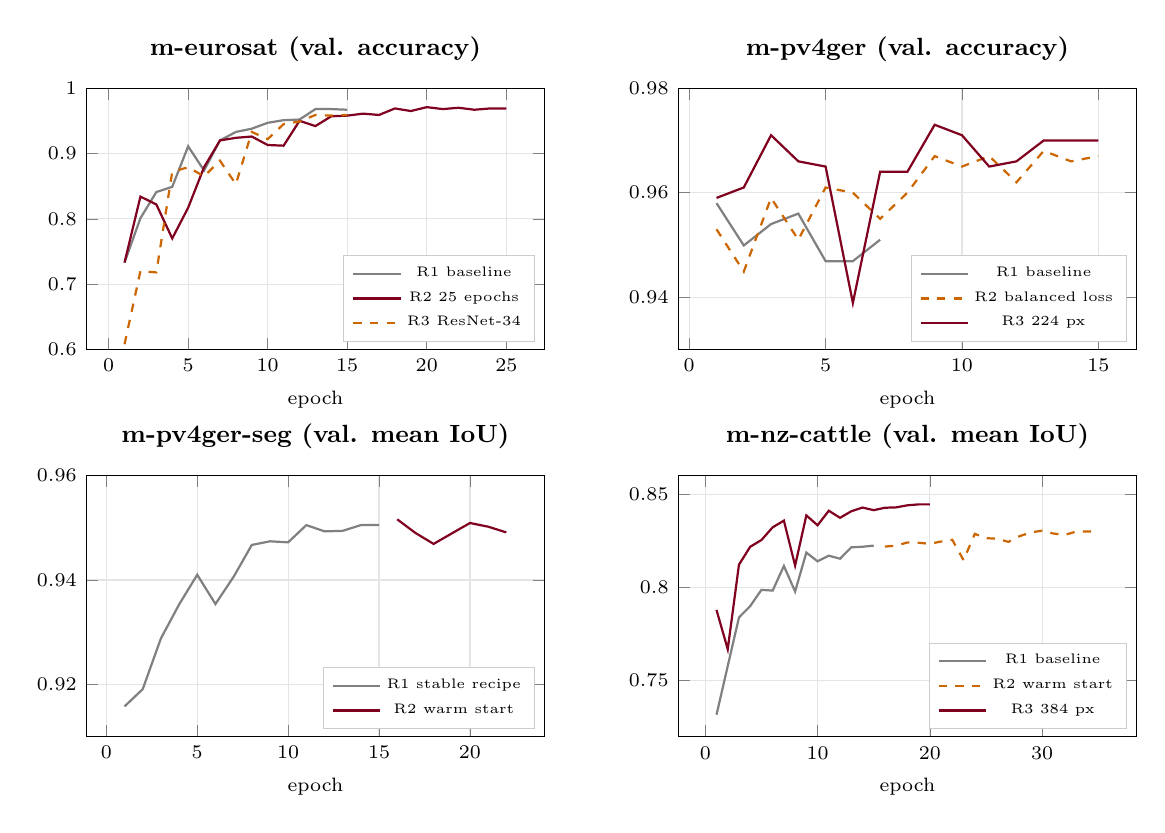
\begin{tikzpicture}
\begin{groupplot}[group style={group size=2 by 2, horizontal sep=1.7cm, vertical sep=1.6cm},
  width=7.4cm, height=4.9cm, xlabel={epoch}, grid=major, grid style={gray!20},
  tick label style={font=\scriptsize}, label style={font=\scriptsize}, title style={font=\small\bfseries},
  legend style={font=\tiny, at={(0.98,0.03)}, anchor=south east, draw=gray!40}, every axis plot/.append style={thick}]
\nextgroupplot[title={m-eurosat (val. accuracy)}, ymin=0.6, ymax=1.0]
\addplot[color=gray, mark=none] coordinates {(1,0.7330)(2,0.8010)(3,0.8410)(4,0.8490)(5,0.9110)(6,0.8740)(7,0.9200)(8,0.9330)(9,0.9380)(10,0.9470)(11,0.9510)(12,0.9520)(13,0.9680)(14,0.9680)(15,0.9670)};
\addplot[color=wine, mark=none] coordinates {(1,0.7330)(2,0.8340)(3,0.8220)(4,0.7700)(5,0.8170)(6,0.8790)(7,0.9200)(8,0.9240)(9,0.9260)(10,0.9130)(11,0.9120)(12,0.9500)(13,0.9420)(14,0.9570)(15,0.9580)(16,0.9610)(17,0.9590)(18,0.9690)(19,0.9650)(20,0.9710)(21,0.9680)(22,0.9700)(23,0.9670)(24,0.9690)(25,0.9690)};
\addplot[color=orange!80!black, dashed, mark=none] coordinates {(1,0.6080)(2,0.7200)(3,0.7180)(4,0.8720)(5,0.8790)(6,0.8650)(7,0.8890)(8,0.8530)(9,0.9330)(10,0.9220)(11,0.9450)(12,0.9490)(13,0.9590)(14,0.9580)(15,0.9590)};
\legend{R1 baseline, R2 25 epochs, R3 ResNet-34}
\nextgroupplot[title={m-pv4ger (val. accuracy)}, ymin=0.93, ymax=0.98]
\addplot[color=gray, mark=none] coordinates {(1,0.9580)(2,0.9499)(3,0.9540)(4,0.9560)(5,0.9469)(6,0.9469)(7,0.9510)};
\addplot[color=orange!80!black, dashed, mark=none] coordinates {(1,0.9530)(2,0.9449)(3,0.9590)(4,0.9510)(5,0.9610)(6,0.9600)(7,0.9550)(8,0.9600)(9,0.9670)(10,0.9650)(11,0.9670)(12,0.9620)(13,0.9680)(14,0.9660)(15,0.9670)};
\addplot[color=wine, mark=none] coordinates {(1,0.9590)(2,0.9610)(3,0.9710)(4,0.9660)(5,0.9650)(6,0.9389)(7,0.9640)(8,0.9640)(9,0.9730)(10,0.9710)(11,0.9650)(12,0.9660)(13,0.9700)(14,0.9700)(15,0.9700)};
\legend{R1 baseline, R2 balanced loss, R3 224 px}
\nextgroupplot[title={m-pv4ger-seg (val. mean IoU)}, ymin=0.91, ymax=0.96]
\addplot[color=gray, mark=none] coordinates {(1,0.9158)(2,0.9191)(3,0.9288)(4,0.9353)(5,0.9410)(6,0.9354)(7,0.9406)(8,0.9467)(9,0.9474)(10,0.9472)(11,0.9505)(12,0.9493)(13,0.9494)(14,0.9505)(15,0.9505)};
\addplot[color=wine, mark=none] coordinates {(16,0.9516)(17,0.9490)(18,0.9469)(19,0.9489)(20,0.9509)(21,0.9502)(22,0.9491)};
\legend{R1 stable recipe, R2 warm start}
\nextgroupplot[title={m-nz-cattle (val. mean IoU)}, ymin=0.72, ymax=0.86]
\addplot[color=gray, mark=none] coordinates {(1,0.7318)(2,0.7579)(3,0.7839)(4,0.7900)(5,0.7987)(6,0.7983)(7,0.8115)(8,0.7978)(9,0.8187)(10,0.8140)(11,0.8170)(12,0.8154)(13,0.8215)(14,0.8218)(15,0.8224)};
\addplot[color=orange!80!black, dashed, mark=none] coordinates {(16,0.8219)(17,0.8224)(18,0.8241)(19,0.8239)(20,0.8234)(21,0.8246)(22,0.8255)(23,0.8146)(24,0.8287)(25,0.8264)(26,0.8261)(27,0.8244)(28,0.8275)(29,0.8295)(30,0.8304)(31,0.8289)(32,0.8281)(33,0.8299)(34,0.8300)(35,0.8300)};
\addplot[color=wine, mark=none] coordinates {(1,0.7879)(2,0.7669)(3,0.8122)(4,0.8218)(5,0.8254)(6,0.8322)(7,0.8358)(8,0.8117)(9,0.8386)(10,0.8333)(11,0.8411)(12,0.8373)(13,0.8408)(14,0.8428)(15,0.8414)(16,0.8427)(17,0.8429)(18,0.8440)(19,0.8445)(20,0.8445)};
\legend{R1 baseline, R2 warm start, R3 384 px}
\end{groupplot}
\end{tikzpicture}
\caption{Per-epoch validation curves of the agent's runs, read from each run's \texttt{history.json}. Warm-start runs are drawn as a continuation of their parent's epochs.}
\label{fig:curves}
\end{figure}

\subsection{EuroSAT: from 75\% to 97\%}

\begin{table}[h]
\centering
\caption{\texttt{m-eurosat} runs (validation accuracy).}
\begin{tabularx}{\linewidth}{@{}lYrr@{}}
\toprule
Run & Hypothesis and change & Val. acc. & $\Delta$ \\
\midrule
manual & 3-layer CNN from scratch, 13 bands, Adam, 5 epochs (before GoTrain) & 75.0\% & -- \\
R1 & Pretrained ResNet-18, 128 px, 15 epochs (agent baseline) & 96.8\% & \up{+21.8} \\
R2 & ``Best epoch was 13/15, so the model may still be improving'': 25 epochs & 97.1\% & \up{+0.3} \\
R3 & Deeper ResNet-34 to separate Herbaceous Vegetation / Annual Crop & 95.9\% & $-1.2$ (rejected) \\
R4 & Scripted refinement: fine-tune R2 at lr $10^{-4}$ & 96.7\% & $-0.4$ (rejected) \\
R5 & Flip TTA on R2 (validation-only comparison) & \textbf{97.2\%} & \up{+0.1} \\
\bottomrule
\end{tabularx}
\end{table}

The single largest gain of the whole project is \textbf{transfer learning with the
13-band adaptation}: +21.8 points over the from-scratch CNN. A bigger backbone was
\emph{worse} on 2{,}000 training images, and the agent kept the smaller model. The
remaining errors are semantic: Herbaceous Vegetation is confused with Annual Crop
(5 of 100 validation images) and vice versa (3 of 100). The same pair is the weak spot on
test, where Annual Crop has the lowest recall (0.88) and Herbaceous Vegetation 0.94.

\subsection{PV4GER classification: fixing missed panels}

\begin{table}[h]
\centering
\caption{\texttt{m-pv4ger} runs (validation accuracy; positive class is 15.6\% of images).}
\begin{tabularx}{\linewidth}{@{}lYrr@{}}
\toprule
Run & Hypothesis and change & Val. acc. & $\Delta$ \\
\midrule
R1 & Pretrained ResNet-18, 128 px. Best epoch was the first; positive recall 0.76 & 95.8\% & -- \\
R2 & ``Low positive recall, 36 false negatives'': class-balanced loss & 96.8\% & \up{+1.0} \\
R3 & ``Panels are small details at 320 px native'': input 224 px & 97.3\% & \up{+0.5} \\
R4 & Scripted refinement of R3 at lr $10^{-4}$ & 97.4\% & \up{+0.1} \\
R5 & Flip TTA on R4 & \textbf{97.5\%} & \up{+0.1} \\
\bottomrule
\end{tabularx}
\end{table}

Accuracy alone hid the real problem. The agent read the confusion matrix, saw that one in
four panels was missed, and attacked recall twice: re-weighting the minority class, then
giving the network more pixels per panel. Validation foreground IoU of the positive class
rose from 0.736 to 0.841. On test, accuracy is 97.9\% with balanced accuracy 0.934; the
remaining weakness is still positive recall (0.869), which our diagnosis also reports
(21 of 153 validation panels missed).

\subsection{PV4GER segmentation: stability first}

\begin{table}[h]
\centering
\caption{\texttt{m-pv4ger-seg} runs (validation mean IoU).}
\begin{tabularx}{\linewidth}{@{}lYrr@{}}
\toprule
Run & Hypothesis and change & Val. mIoU & $\Delta$ \\
\midrule
R0 & U-Net, 256 px, lr $3\times10^{-4}$, mixed precision & failed & non-finite loss \\
R1 & ``Instability from AMP or high learning rate'': lr $10^{-4}$, AMP off & 0.9505 & -- \\
R2 & ``Best epoch was the last'': warm start at lr $5\times10^{-5}$ & 0.9516 & \up{+0.0011} \\
R3 & Scripted refinement at lr $1.7\times10^{-5}$ & 0.9519 & \up{+0.0003} \\
R4 & Flip TTA on R3 & \textbf{0.9526} & \up{+0.0007} \\
\bottomrule
\end{tabularx}
\end{table}

The first attempt diverged. The engine detected the non-finite loss, failed the run
cleanly (the run is still recorded) and the agent diagnosed a plausible cause and fixed
it on the next attempt. After that, the problem was largely solved by the first stable
recipe; later steps added small, measured gains. Foreground IoU on test is 0.921.

\subsection{NZ cattle: small objects need pixels}

\begin{table}[h]
\centering
\caption{\texttt{m-nz-cattle} runs (validation mean IoU; cattle are 2.2\% of pixels).}
\begin{tabularx}{\linewidth}{@{}lYrr@{}}
\toprule
Run & Hypothesis and change & Val. mIoU & $\Delta$ \\
\midrule
R1 & Pretrained U-Net, 256 px, CE + Dice & 0.8224 & -- \\
R2 & ``Best epoch was the last'': warm start, lr $10^{-4}$, 20 epochs & 0.8304 & \up{+0.0080} \\
R3 & ``Cattle are $\sim$2\% of pixels'': 384 px input, trained from pretrained & 0.8445 & \up{+0.0141} \\
R4 & Scripted refinement of R3 at lr $10^{-4}$ & 0.8453 & \up{+0.0008} \\
R5 & Flip TTA on R4 & \textbf{0.8476} & \up{+0.0023} \\
\bottomrule
\end{tabularx}
\end{table}

This is the hardest task: tiny objects, 524 training images and only 66 for validation.
Resolution was the decisive lever. Our post-hoc diagnosis of the final model counts 2{,}559
annotated animals in validation and finds 99\% of the small ones and 96\% of the large ones
at the object level, with a predicted area $1.05\times$ the true area, so the remaining IoU
gap is mostly about exact boundaries of rasterised annotations rather than missed animals.

\subsection{What worked across tasks}

\begin{table}[h]
\centering
\caption{Measured effect of each lever (validation, our runs).}
\begin{tabularx}{\linewidth}{@{}lYl@{}}
\toprule
Lever & Evidence & Verdict \\
\midrule
ImageNet pretraining + band adaptation & EuroSAT 75.0\% $\to$ 96.8\% & essential \\
Higher input resolution & PV4GER +0.5 pt; cattle +0.0141 mIoU & helps small objects \\
Class-balanced loss & PV4GER +1.0 pt, positive recall up & helps rare classes \\
Training longer / warm start & EuroSAT +0.3 pt; cattle +0.0080; seg +0.0011 & helps if still improving \\
Lower-LR refinement & +0.0003 to +0.001 on 3 tasks, $-0.4$ pt on EuroSAT & small, not always \\
Flip TTA & better on \textbf{4 of 4} tasks (+0.0007 to +0.0023) & cheap, consistent \\
Deeper backbone (ResNet-34) & EuroSAT $-1.2$ pt & rejected \\
\bottomrule
\end{tabularx}
\end{table}

All four final models used about 64 GPU-minutes of training on one T4 in total. Speed
came from pretrained backbones, cached inputs, early stopping and a hard experiment budget.

% ===========================================================================
\section{Final Test Results}
% ===========================================================================

\begin{table}[h]
\centering
\caption{Full test metrics of the four frozen models.}
\begin{tabular}{@{}lrrrrr@{}}
\toprule
Task & Accuracy & Balanced acc. & Macro-F1 & Mean IoU & Foreground IoU \\
\midrule
\texttt{m-eurosat} & \textbf{0.9570} & 0.9570 & 0.9569 & 0.9189 & -- \\
\texttt{m-pv4ger} & \textbf{0.9790} & 0.9340 & 0.9573 & 0.9197 & 0.8636 \\
\texttt{m-pv4ger-seg} & 0.9853 & 0.9749 & 0.9749 & \textbf{0.9514} & 0.9206 \\
\texttt{m-nz-cattle} & 0.9913 & 0.9202 & 0.9084 & \textbf{0.8439} & 0.6967 \\
\bottomrule
\end{tabular}
\end{table}

\textbf{Validation versus test.} The gaps are $-1.5$ points (EuroSAT), $+0.4$ points (PV4GER),
$-0.0012$ (PV4GER-seg) and $-0.0037$ (cattle). Small gaps on three tasks indicate that selecting
on validation did not overfit; EuroSAT's larger drop is consistent with many sequential
choices made on one 1{,}000-image validation set.

\textbf{Traceability.} Every score above links to a selected run ID, its checkpoint SHA-256,
the evaluation time and the original \texttt{test-result.json}, and the metrics were
re-verified from the saved confusion matrices (Figure~\ref{fig:dash}).

\begin{figure}[h]
\centering
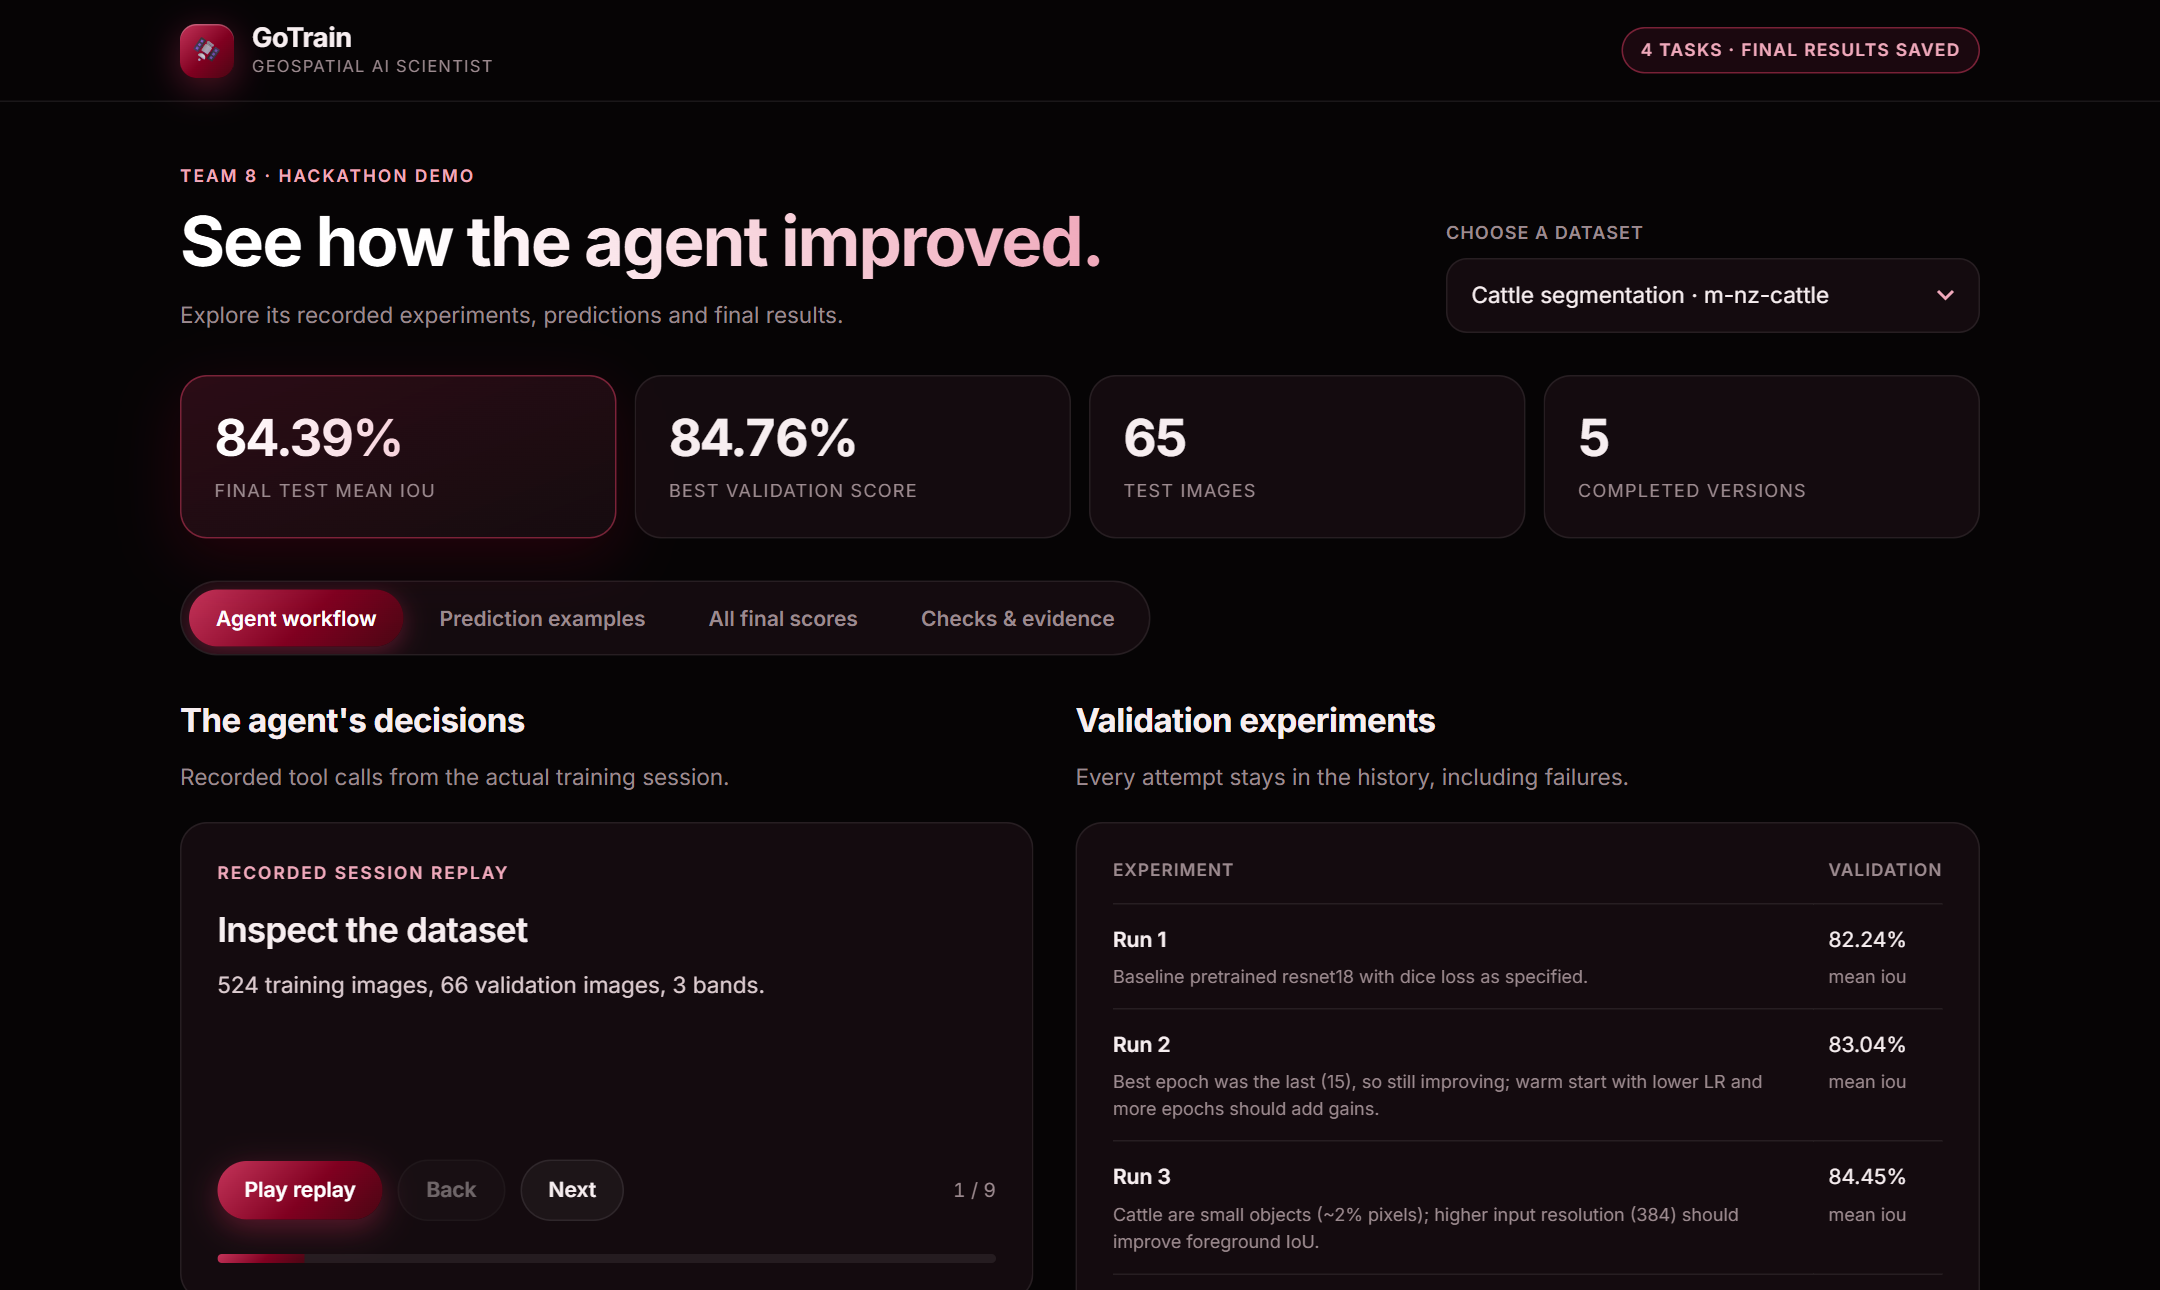
\includegraphics[width=0.49\linewidth]{figures/dashboard-overview.png}\hfill
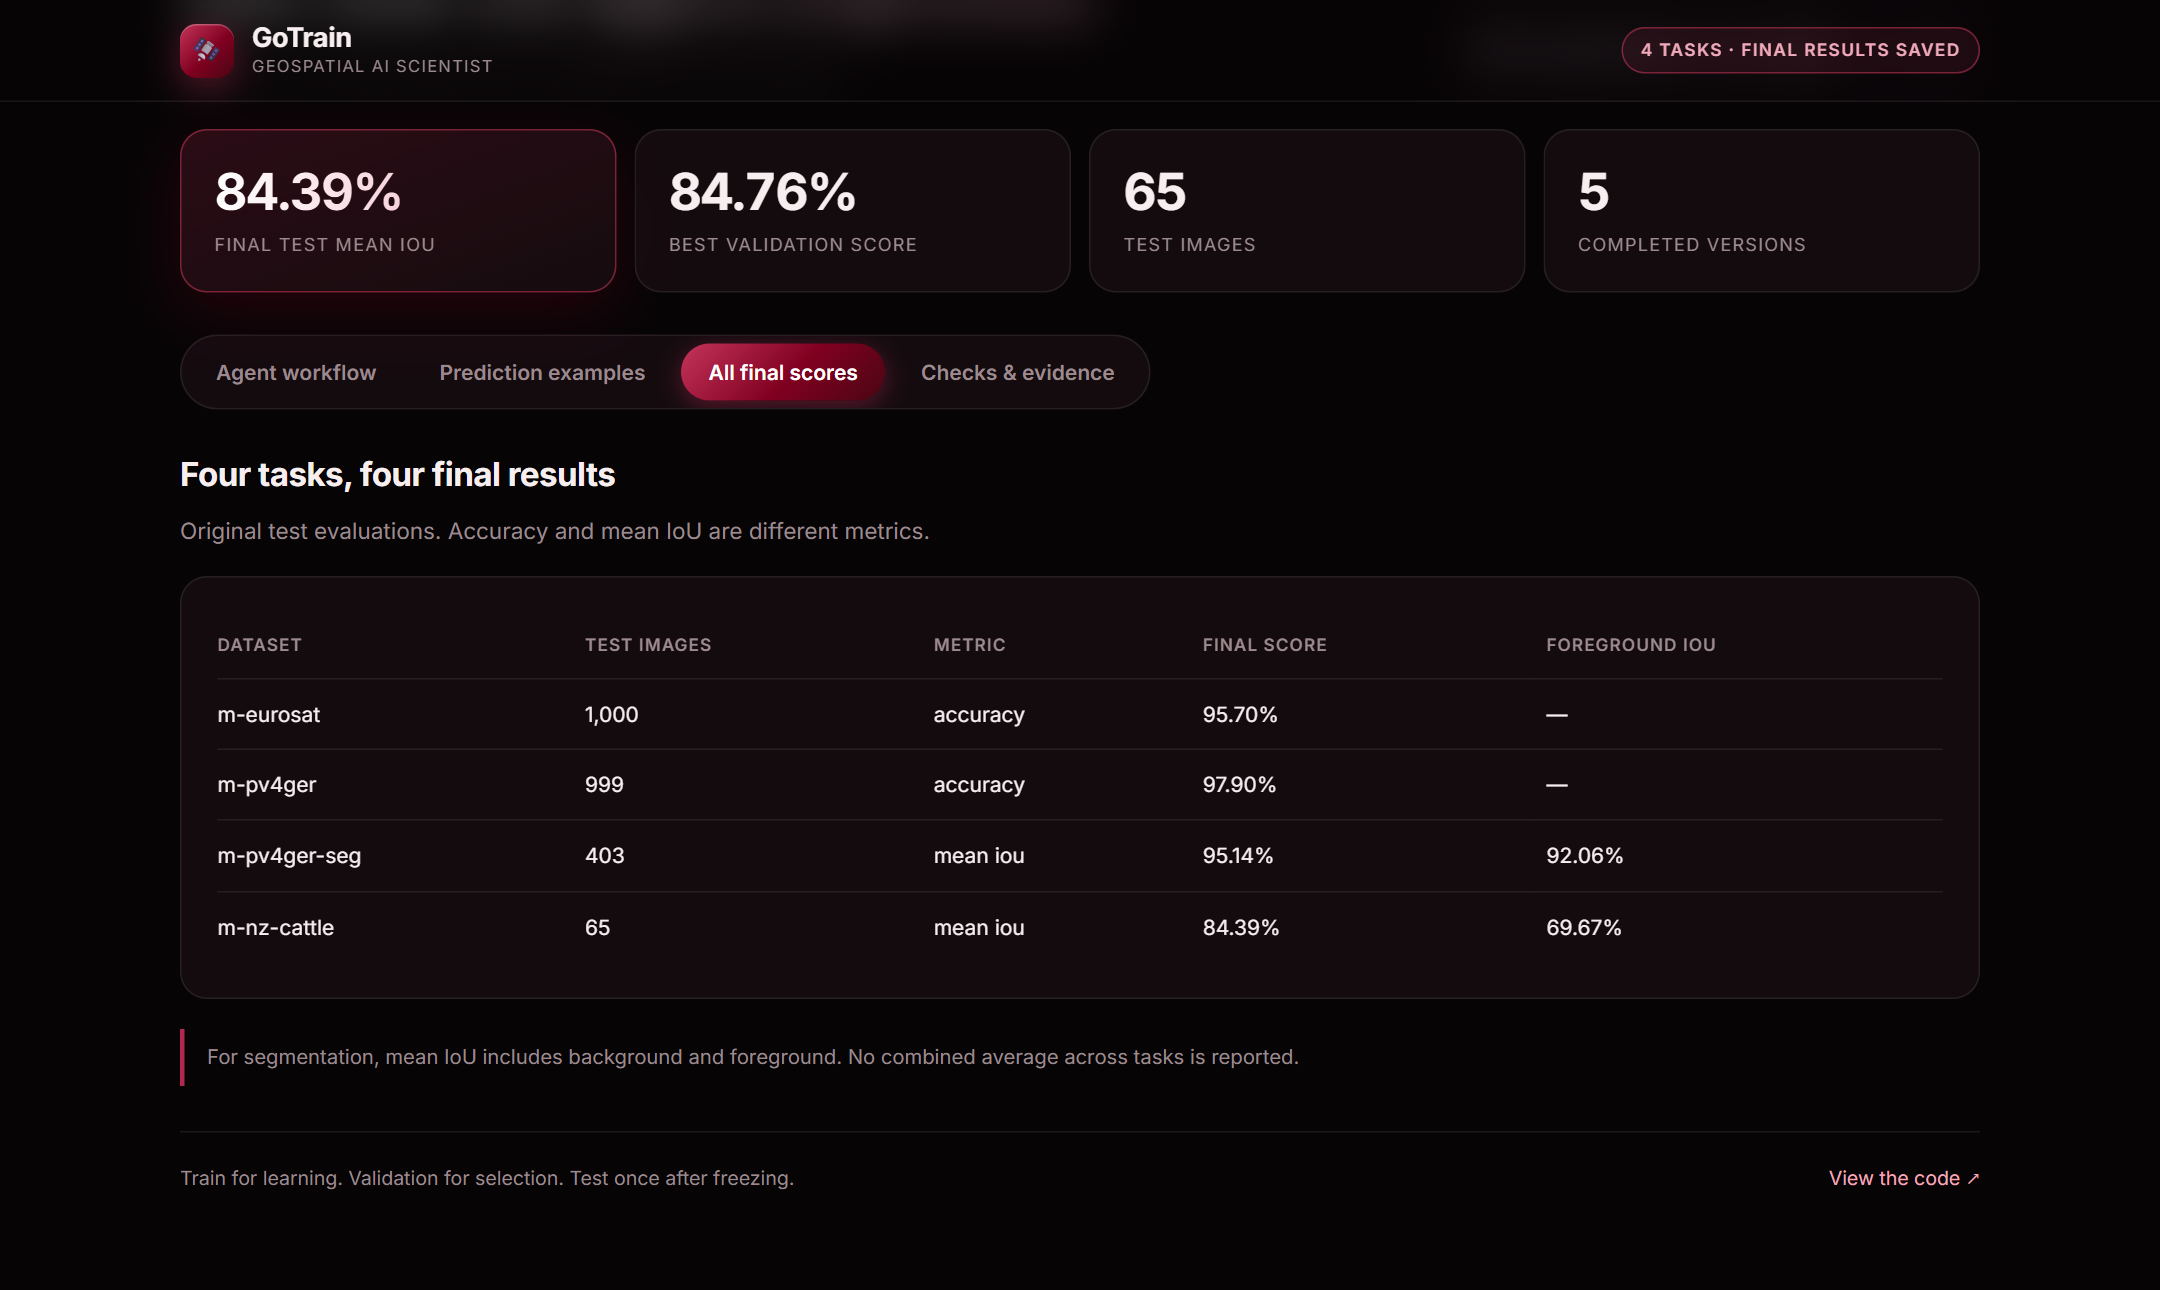
\includegraphics[width=0.49\linewidth]{figures/dashboard-results.png}
\caption{Results dashboard built from the exported evidence: per-task metrics and agent replay (left), all four final scores (right).}
\label{fig:dash}
\end{figure}

% ===========================================================================
\section{What Makes GoTrain Innovative}
% ===========================================================================

The scored runs above already used hypothesis-driven experiments. On top of them we built
the features that turn GoTrain from a tuning loop into an \textbf{AI scientist}. They
were built after the scored runs and were \emph{not} used to produce the final scores;
they were run on the frozen models using validation data only.

\subsection{Error-driven diagnosis}

\begin{definition}{Object-level detection by size}{objects}
Each true foreground mask is split into 8-connected components (one component per object).
An object is \emph{detected} if at least 50\% of its pixels are predicted as foreground.
Objects are grouped into small / medium / large by the terciles of their areas, and the
detection rate is reported per group.
\end{definition}

\texttt{diagnose\_errors} also reports predicted-to-true foreground area, false positives on
images with no target, the most-confused class pairs, the weakest class recall, and the
worst validation images as pictures. It then lists \emph{candidate levers}, for example
``small objects detected less often $\Rightarrow$ try \texttt{focus\_crops} or a larger
image size''. The agent must quote one of these measured numbers in its next hypothesis.

\begin{figure}[h]
\centering

\includegraphics[width=0.62\linewidth]{figures/diagnosis-m-pv4ger-seg-worst.png}
\caption{A worst validation image found by \texttt{diagnose\_errors} on PV4GER-seg: input, true mask, prediction. Its diagnosis: small panels found 88\% of the time versus 99\% for larger ones.}
\end{figure}

\subsection{Targeted fixes and verdicts}

\texttt{focus\_crops} is a new segmentation option: half of the training samples are cropped
to a half-size window around a random foreground pixel (with jitter) and resized back, so
objects appear twice as large; image and mask stay aligned. After every experiment the
tool returns a verdict, \texttt{kept} only if the run strictly beats the previous best
validation score, together with the minutes and attempts left.

\subsection{Memory across datasets}

\begin{definition}{Lesson}{lesson}
A lesson is the recipe difference between a run and the best run it had to beat, together
with the measured validation change and a verdict (\emph{kept}, \emph{rejected} or
\emph{failed}). Lessons are derived mechanically from run records, so they cannot be
invented. The agent can add \emph{insights}, but each must cite run IDs from the task.
\end{definition}

Before its first experiment on a new dataset, the agent calls \texttt{recall\_lessons} and
receives lessons from other tasks (same problem type first), a scoreboard per lever and
the winning recipe of each similar task. Lessons are hints to re-test, never results.
Reconstructed from our real runs, the memory holds 15 lessons across the four tasks;
for instance flip TTA was kept 4 of 4 times, and $256\to384$ px gave $+0.0142$ mIoU on cattle.

\begin{figure}[h]
\centering
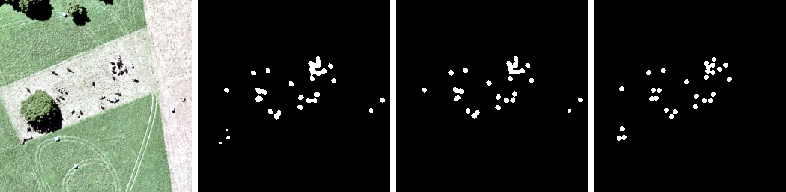
\includegraphics[width=0.49\linewidth]{figures/showcase-m-nz-cattle-2.png}\hfill
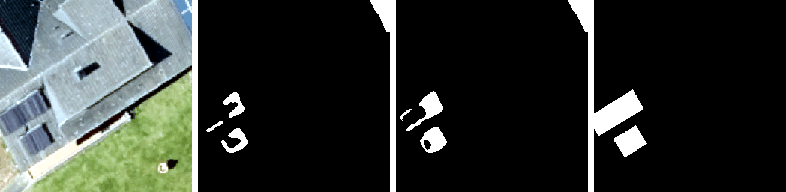
\includegraphics[width=0.49\linewidth]{figures/showcase-m-pv4ger-seg-2.png}
\caption{Before and after on the first model's hardest validation images (input, first model, selected model, true mask). Cattle: foreground IoU 0.51 $\to$ 0.56. Solar panels: 0.30 $\to$ 0.45. These images were chosen because they were the worst, not because they improved; one of the three PV4GER-seg examples stayed at 0.}
\end{figure}

\subsection{A product, not a notebook}

\begin{itemize}
  \item \textbf{Chat interface.} Type ``find cattle in aerial photos, 45 minutes, 3
  experiments''; GoTrain parses the task, budget and number of experiments (and asks when
  unclear), starts the agent and streams every step as a chat message (Figure~\ref{fig:ui}).
  \item \textbf{Model registry.} All 20 model versions with lineage, checksums and badges
  (best, published, verified, frozen); one-click publish and restore-and-verify; an audited
  storage log. In our workspace, 11 versions are published and 4 were restored with every
  checksum matched.
  \item \textbf{Demo video and dashboard} built from the recorded evidence.
  \item \textbf{GoPilot-ready.} \texttt{python -m gotrain.mcp\_server} exposes inspection,
  training, diagnosis, memory, comparison and model upload/download as MCP tools, with no
  test-split access.
\end{itemize}

\begin{figure}[h]
\centering
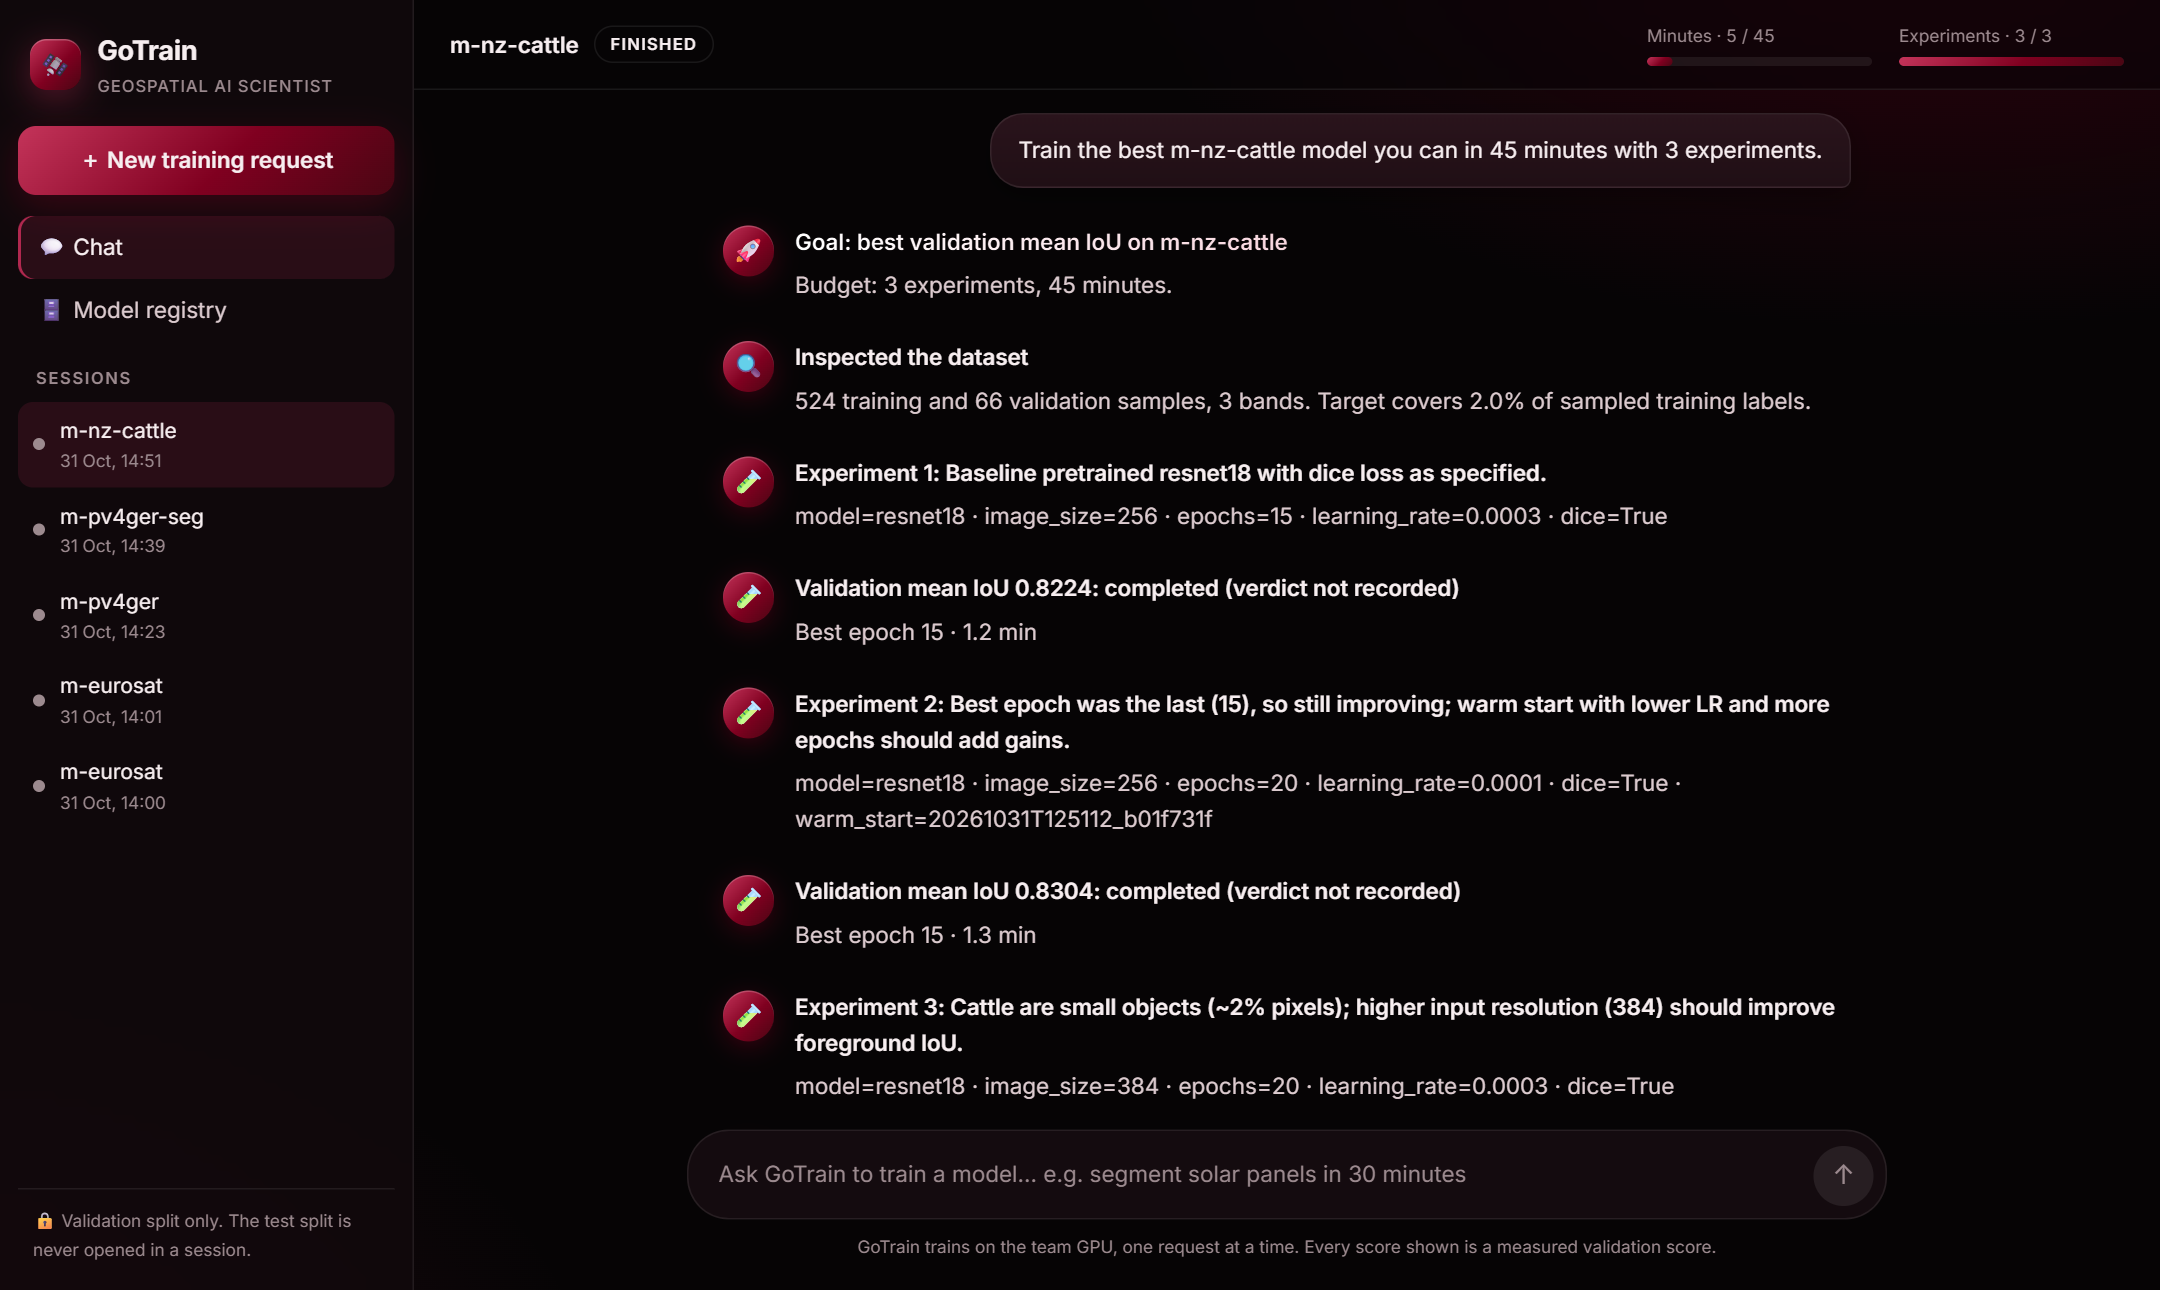
\includegraphics[width=0.49\linewidth]{figures/ui-session.png}\hfill
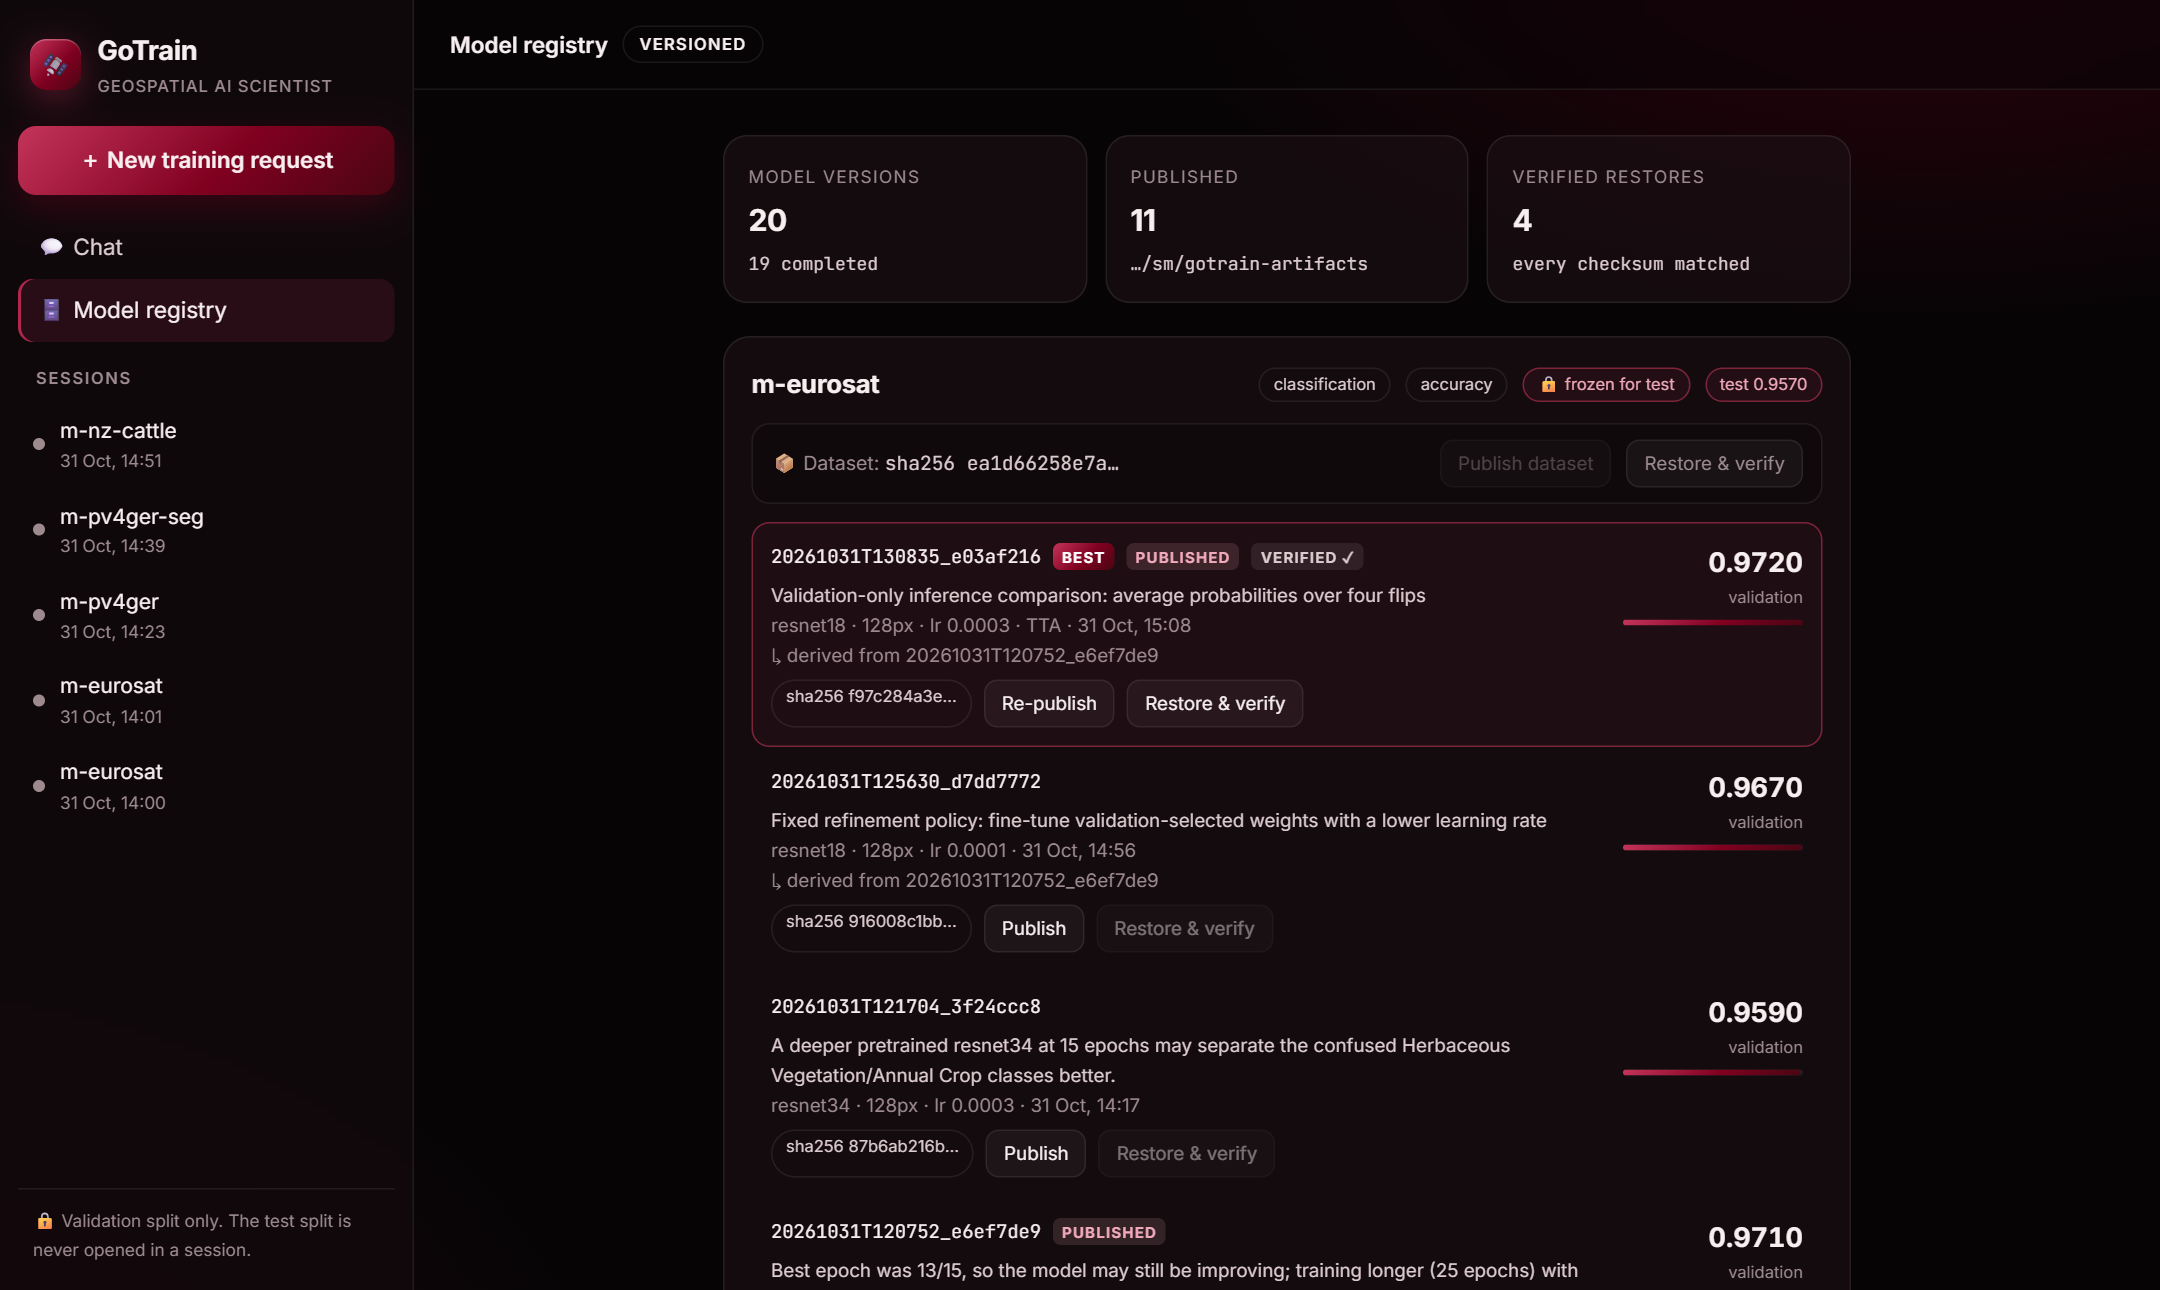
\includegraphics[width=0.49\linewidth]{figures/ui-registry.png}\\[0.6em]
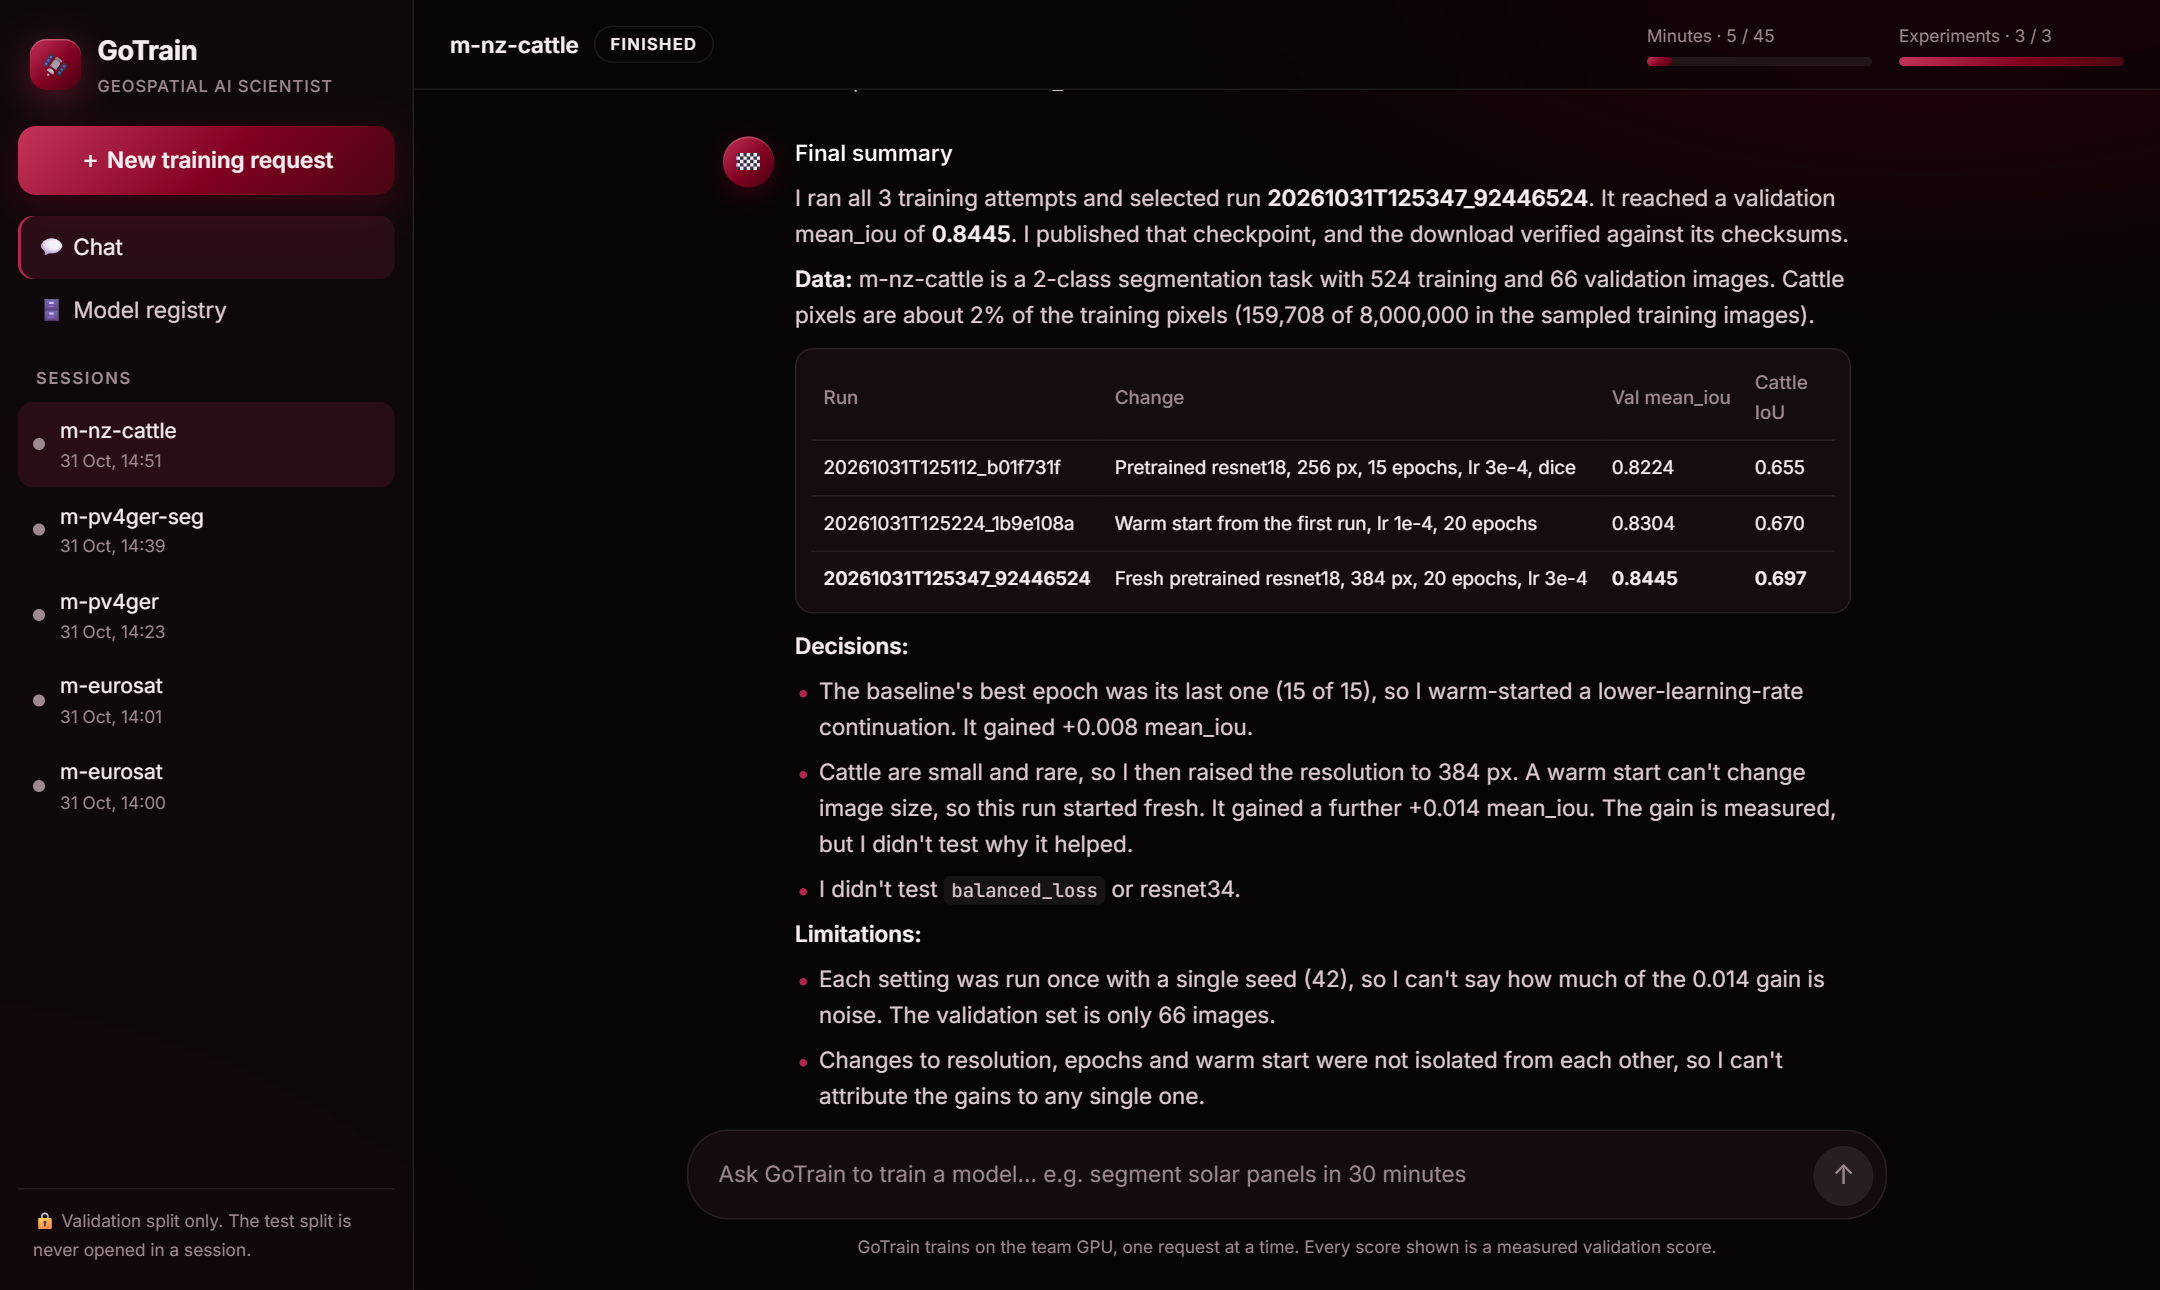
\includegraphics[width=0.49\linewidth]{figures/ui-summary.png}\hfill
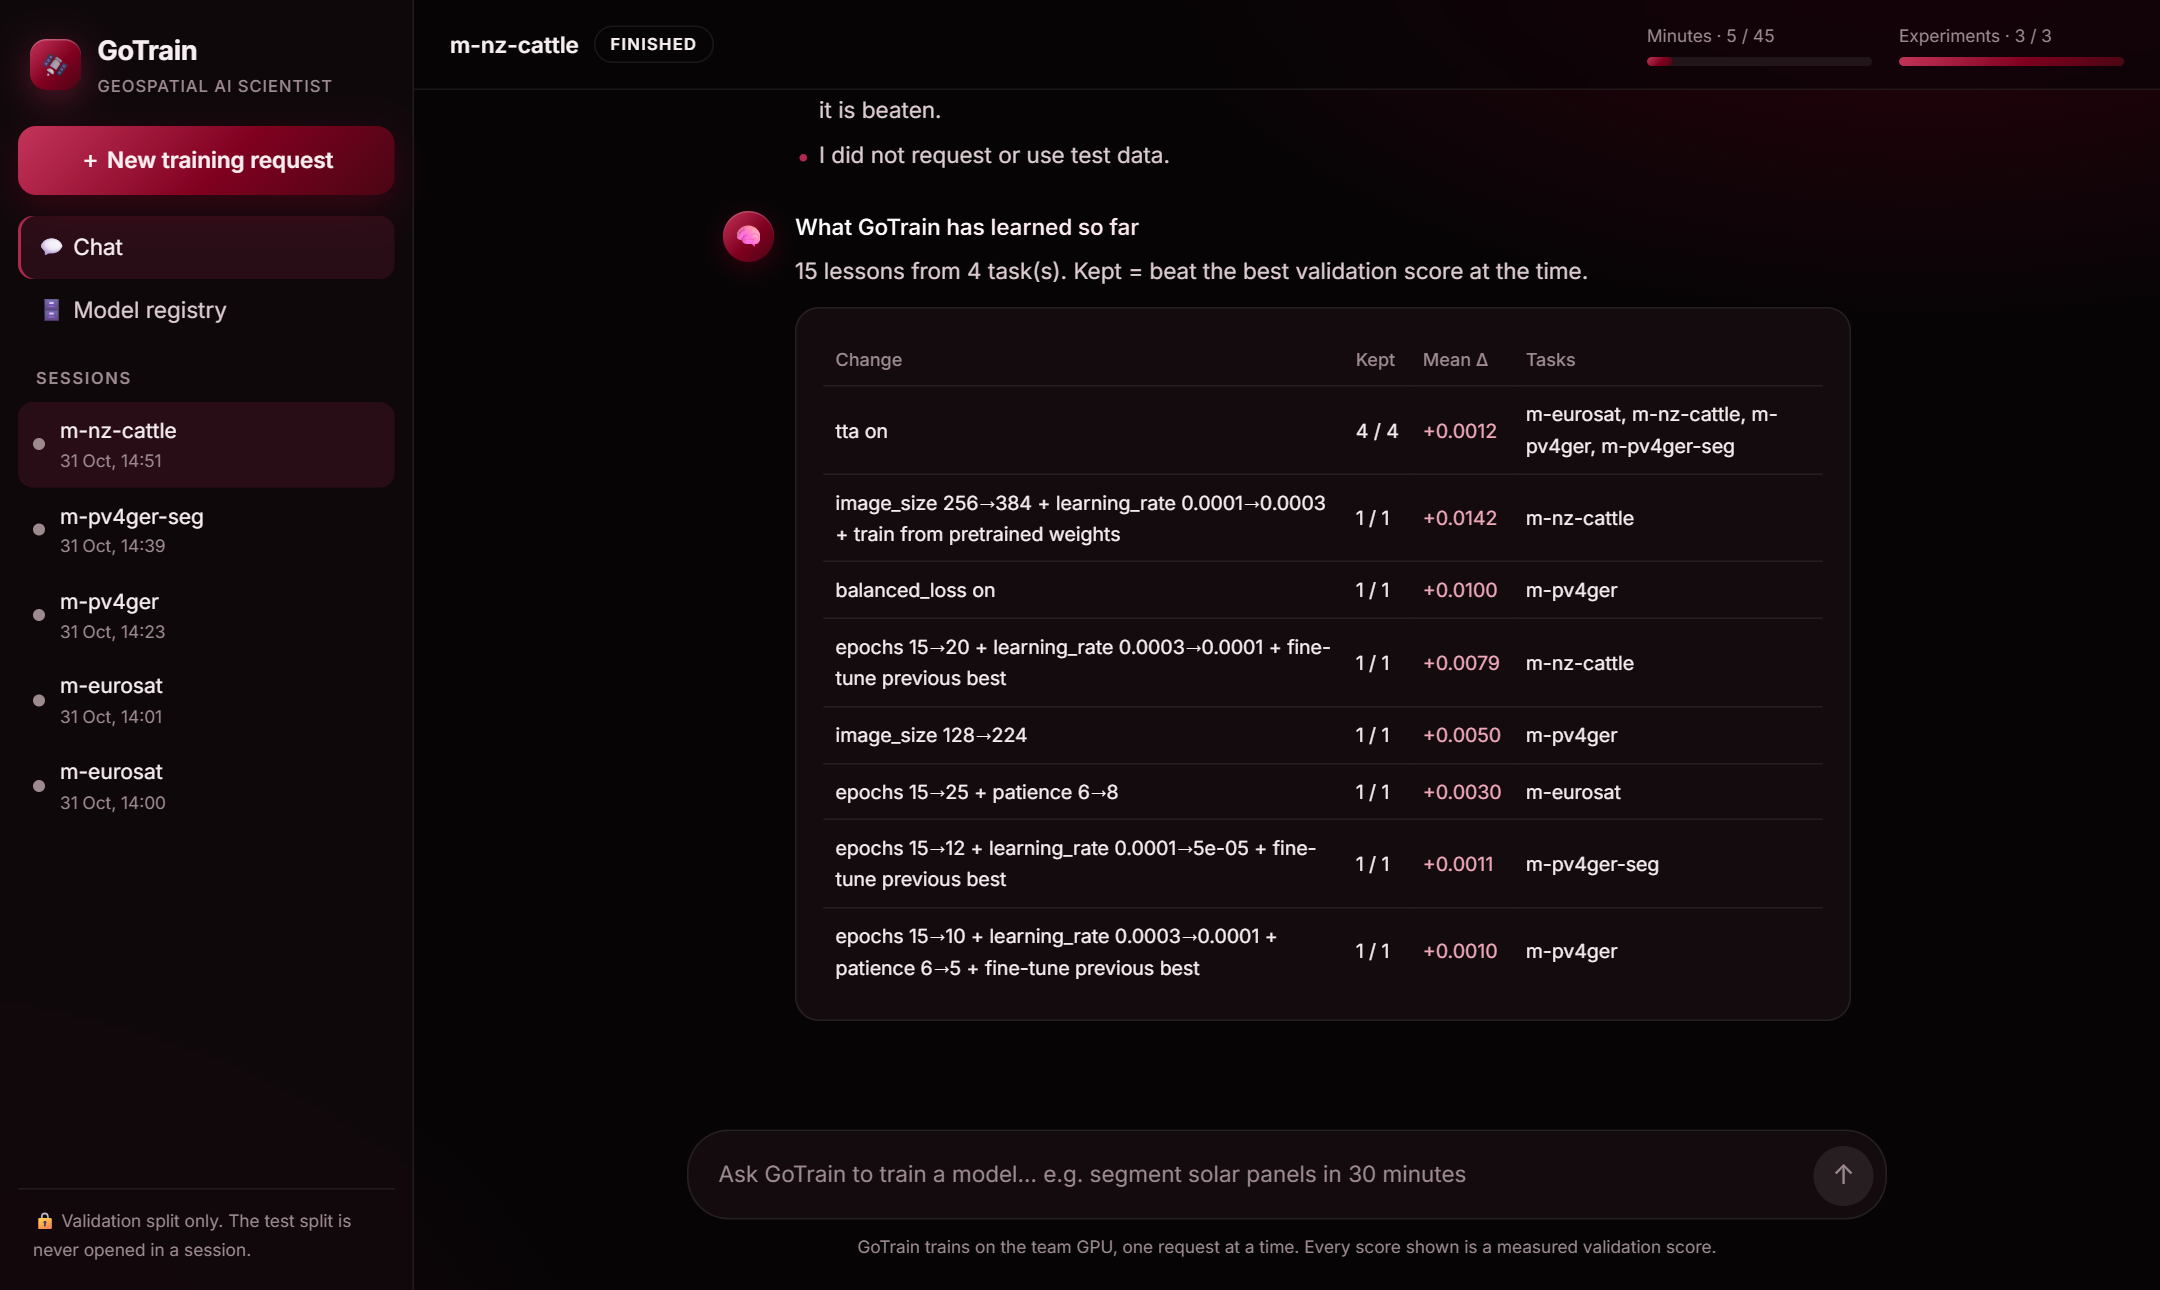
\includegraphics[width=0.49\linewidth]{figures/ui-memory.png}
\caption{The GoTrain chat app: a real agent session (top left), the model registry (top right), the agent's own final summary (bottom left) and the cross-task memory scoreboard (bottom right).}
\label{fig:ui}
\end{figure}

% ===========================================================================
\section{Evaluation Integrity and Engineering}
\label{sec:integrity}
% ===========================================================================

\subsection{Test exactly once}

\texttt{gotrain finalize TASK --confirm-test-once} (1) selects the best validation run,
(2) writes \texttt{final-selection.json} with an exclusive create, (3) verifies the
checkpoint hash and the dataset fingerprint, (4) writes \texttt{test-started.json}, again with
an exclusive create, \emph{before} the first test sample is read, and (5) evaluates. A second
call fails before touching the test split, a crash after step 4 stays locked, and training on
a frozen task is refused. A file lock also prevents two GPU jobs from running at the same time.

\subsection{Reproducibility and provenance}

Each run stores its recipe, seed, hypothesis, git commit, package versions, GPU name, dataset
fingerprint (hashes of the task files), normalisation sample indices and the full per-epoch
history. Checkpoints are written atomically and hashed; warm starts and inference variants
record their parent's hash, so model lineage is verifiable.

\subsection{Testing}

34 automated tests run on synthetic fixtures in CI: metrics, the train/valid-only guard,
train-only normalisation, mask alignment, focus crops, global IoU, checkpoint corruption,
once-only finalisation, warm-start lineage, TTA un-flipping, diagnosis and lessons, the
agent's budget and logs with a mocked model, the chat server, the registry, and the
dashboard's escaping of untrusted text.

% ===========================================================================
\section{Honest Limitations}
% ===========================================================================

\begin{remarkbox}
We prefer to state these ourselves; they are also written in our logs and README.
\end{remarkbox}

\begin{itemize}
  \item \textbf{Single seed.} Each setting ran once (seed 42); differences of $\sim$0.001
  are within noise, especially on 66 cattle validation images.
  \item \textbf{Confounded changes.} Some runs changed several settings together (for
  example resolution, learning rate and initialisation for cattle R3), so a gain cannot be
  attributed to one setting alone.
  \item \textbf{Scripted steps.} The refinement (R4) and TTA (R5) steps were fixed policies,
  not agent decisions; we report them separately.
  \item \textbf{New features after scoring.} Diagnosis, focus crops, verdicts and memory did
  not produce the final scores; memory was reconstructed from the runs after freezing.
  \item \textbf{Comparison protocol.} We did not reproduce the GEO-Bench paper's exact
  protocol (budget, seeds, pretraining), so we do not claim a ranking against it.
  \item \textbf{Deployment.} Storage was verified on the filesystem; cloud object storage
  and a live GoPilot deployment were not exercised.
\end{itemize}

% ===========================================================================
\section{What We Would Build Next at RASID}
% ===========================================================================

\begin{enumerate}
  \item \textbf{Ship GoTrain as an MCP server inside GoPilot}, with authentication and
  cloud object storage for datasets and model versions.
  \item \textbf{Close the scientist loop on new data}: run diagnosis $\to$ targeted fix
  (\texttt{focus\_crops}, resolution, balancing) $\to$ verdict end to end, and measure
  how much recalled memory shortens the search on a fresh dataset.
  \item \textbf{Statistical rigour}: multiple seeds and confidence intervals before a change
  is \emph{kept}; isolate one change per experiment.
  \item \textbf{Stronger backbones}: geospatial foundation models pretrained on
  multispectral imagery, compared under the same protocol.
  \item \textbf{Search that branches}: explore several promising recipes in parallel (tree
  search) when more than one GPU is available.
\end{enumerate}

\divider

\textbf{In one sentence:} GoTrain trains strong geospatial models on its own, explains every
decision with a measured hypothesis, learns from one dataset to the next, and proves each
final score with an auditable, test-once trail.

% ===========================================================================
\section{Appendix: Reproduce and Verify}
% ===========================================================================

\subsection{Commands}

\begin{verbatim}
python -m pip install -e '.[dev]'
python -m pytest -q                                   # 34 tests
python -m gotrain prepare m-nz-cattle
python -m gotrain agent m-nz-cattle --experiments 3 --minutes 45
python -m gotrain diagnose m-nz-cattle                # validation only
python -m gotrain learn m-nz-cattle                   # lessons from runs
python -m gotrain ui                                  # chat + registry
python -m gotrain finalize m-nz-cattle --confirm-test-once
python -m gotrain export --out submission
\end{verbatim}

\subsection{Frozen model versions}

\begin{table}[h]
\centering
\begin{tabular}{@{}ll@{}}
\toprule
Task & Selected run (validation-chosen, then tested once) \\
\midrule
\texttt{m-eurosat} & \run{20261031T130835\_e03af216} (R2 + flip TTA) \\
\texttt{m-pv4ger} & \run{20261031T130848\_2e474ff8} (R4 + flip TTA) \\
\texttt{m-pv4ger-seg} & \run{20261031T130907\_dd275c19} (R3 + flip TTA) \\
\texttt{m-nz-cattle} & \run{20261031T130927\_b6c58559} (R4 + flip TTA) \\
\bottomrule
\end{tabular}
\end{table}

Code: \url{https://github.com/mastercoder67/GoTrain-Hackathon}.

\end{document}
